\documentclass[tikz,border=8pt]{standalone}
\usepackage{amsmath,amssymb}
\usepackage{tikz}
\usetikzlibrary{automata,positioning,arrows.meta}

\begin{document}
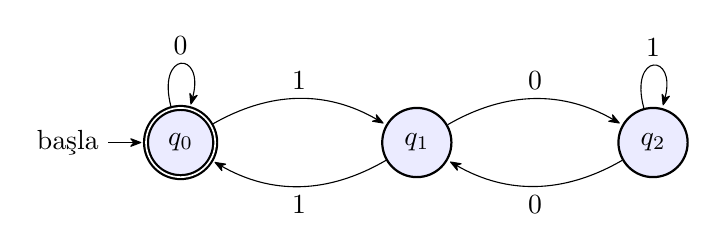
\begin{tikzpicture}[
  shorten >=1pt, node distance=3cm, on grid, auto,
  >={Stealth[round]}, every state/.style={thick, fill=blue!8},
  initial text={başla},
]
  \node[state, initial, accepting] (q0) {$q_0$};
  \node[state] (q1) [right=of q0] {$q_1$};
  \node[state] (q2) [right=of q1] {$q_2$};
  \path[->]
    (q0) edge [loop above] node {0} ()
         edge [bend left]  node {1} (q1)
    (q1) edge [bend left]  node {1} (q0)
         edge [bend left]  node {0} (q2)
    (q2) edge [loop above] node {1} ()
         edge [bend left]  node {0} (q1);
\end{tikzpicture}
\end{document}
